\chapter{IPv4 Addressing: Part 1}\label{ipv4-addressing-part-1}

OSI MODEL - NETWORK LAYER (Layer 3)

\begin{itemize}
\tightlist
\item
  Provides connectivity between end hosts on DIFFERENT networks (ie:
  outside of the LAN)
\item
  Provides logical addressing (IP addresses)
\item
  Provides path selection between SOURCE and DESTINATION
\item
  ROUTERS operate at LAYER 3
\end{itemize}

\section{Routing}\label{routing}

SWITCHES (Layer 2 Devices) do no separate different networks. They
connect and EXPAND networks within the same LAN.

By adding a ROUTER, however, between two SWITCHES, you create a SPLIT in
the network; each with it's own network IP address.

Example: 192.168.1.0/24 (255.255.255.0) 192.168.2.0/24 (255.255.255.0)

\begin{figure}
\centering
\pandocbounded{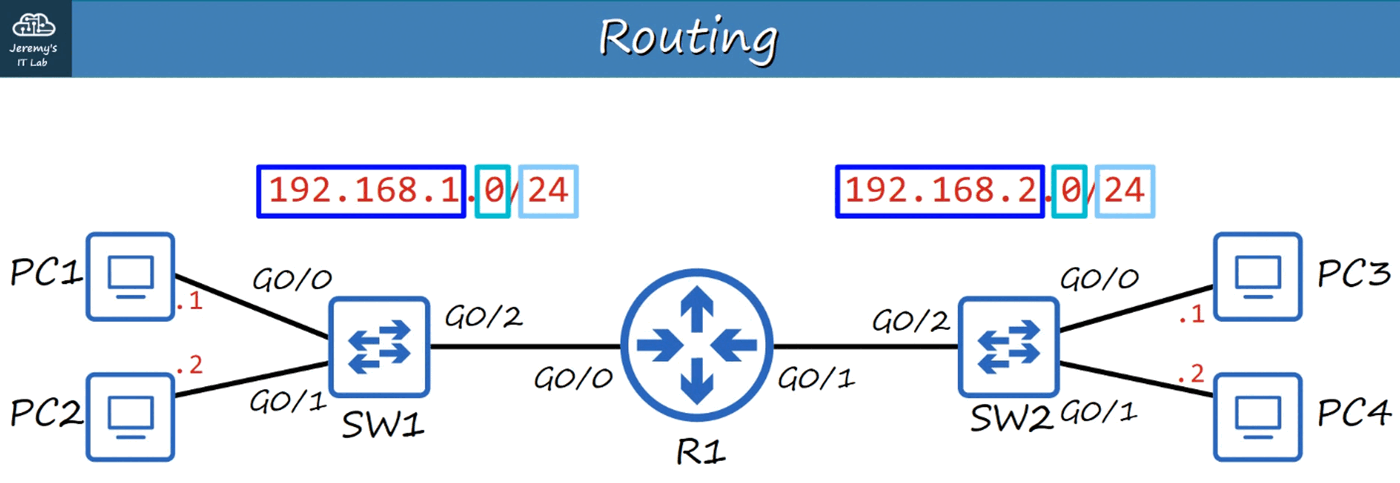
\includegraphics[keepaspectratio,alt={image}]{images/07-ipv4-addressing-part1/img-001.png}}
\end{figure}

ROUTERS have unique IP Addresses for EACH of their interface
connections, depending on their location.

The IP Address for the ROUTER's G0/0 Interface is: 192.168.1.254/24

The IP Address for the ROUTER's G0/1 Interface is: 192.168.2.254/24

\begin{figure}
\centering
\pandocbounded{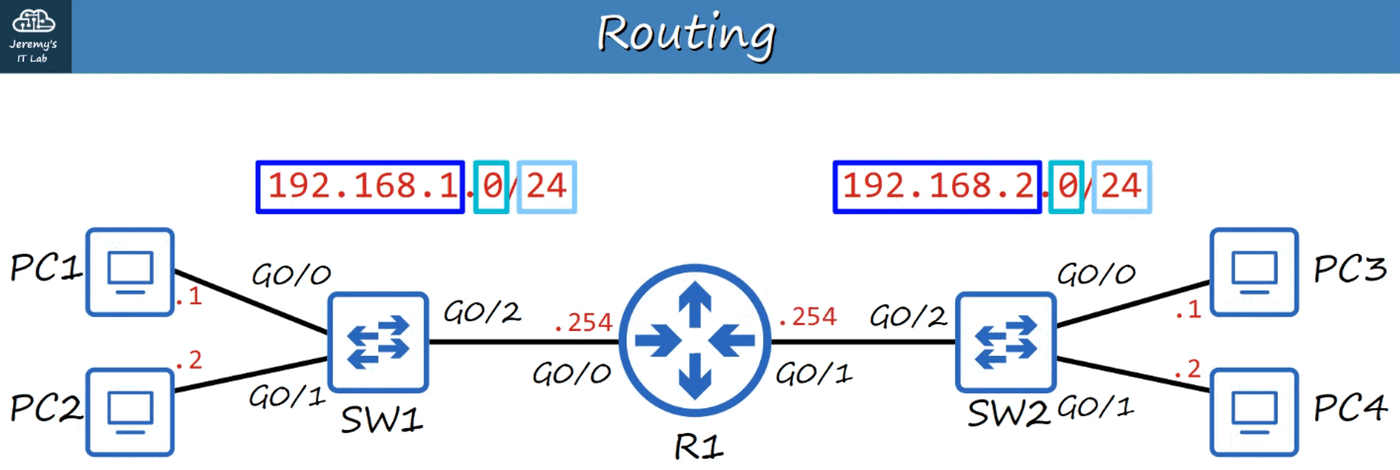
\includegraphics[keepaspectratio,alt={image}]{images/07-ipv4-addressing-part1/img-002.png}}
\end{figure}

The IP Address depends on network address of the LAN it is connects to.

The NETWORK portion of given IP Address will be the same for all HOSTS
on a given LAN.

Example:

192.168.1.100 192.168.1.105 192.168.1.205

All of these addresses are on the SAME Network because the NETWORK
PORTION of their IP Address is the same (192.168.1) while the HOST part
(100,105,205) is UNIQUE!

When a BROADCAST message hits a ROUTER, it does NOT continue onward. It
stays within the LOCAL LAN (Switch/Hosts).

IPv4 HEADER

\begin{figure}
\centering
\pandocbounded{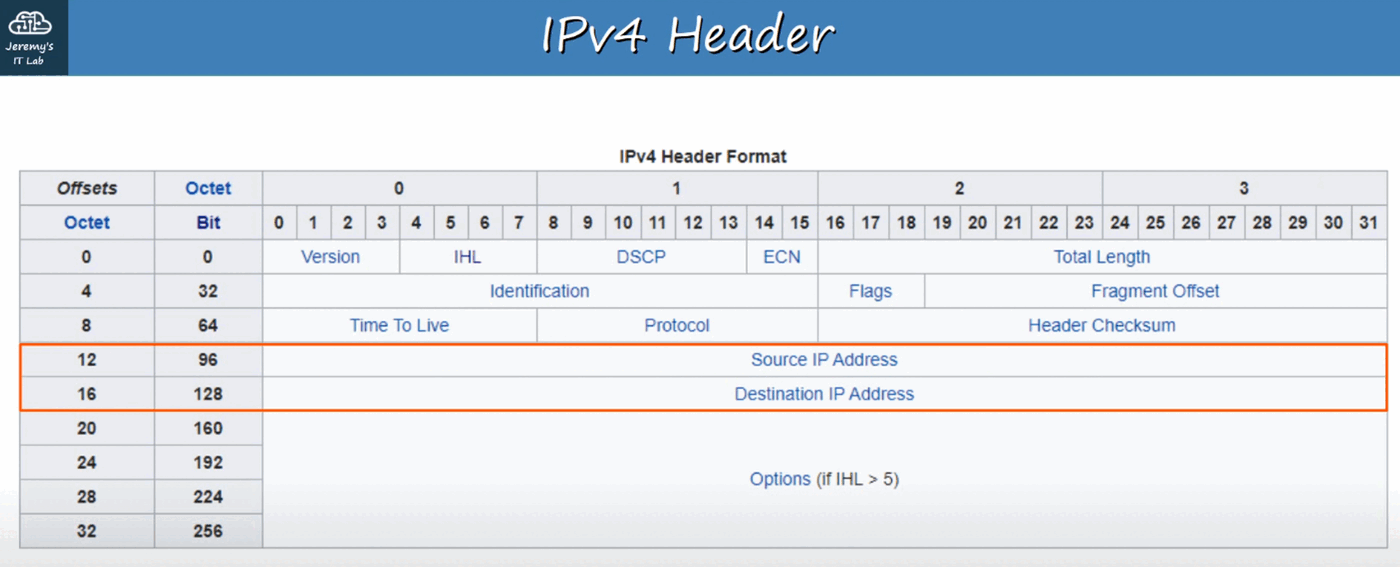
\includegraphics[keepaspectratio,alt={image}]{images/07-ipv4-addressing-part1/img-003.png}}
\end{figure}

IP (or Internet Protocol) is the primary Layer 3 protocol in use today.
Version 4 is the version in use in most networks.

IPv4 Headers contain MORE fields than the ETHERNET header.

IPv4 Headers contain a SOURCE IP Address and DESTINATION IP Address
field.

This FIELD is 32-bits(4-bytes) in length (0-31)

192.168.1.254 (each decimal number represents 8 bits)

Translated to Binary:

11000000 . 10101000 . 00000001 . 11111110

EACH of these 8 bit groups are referred to as an OCTET

Since Binary is difficult to read for people, we use the Dotted Decimal
format.

REVIEW of DECIMAL and HEXADECIMAL

\begin{figure}
\centering
\pandocbounded{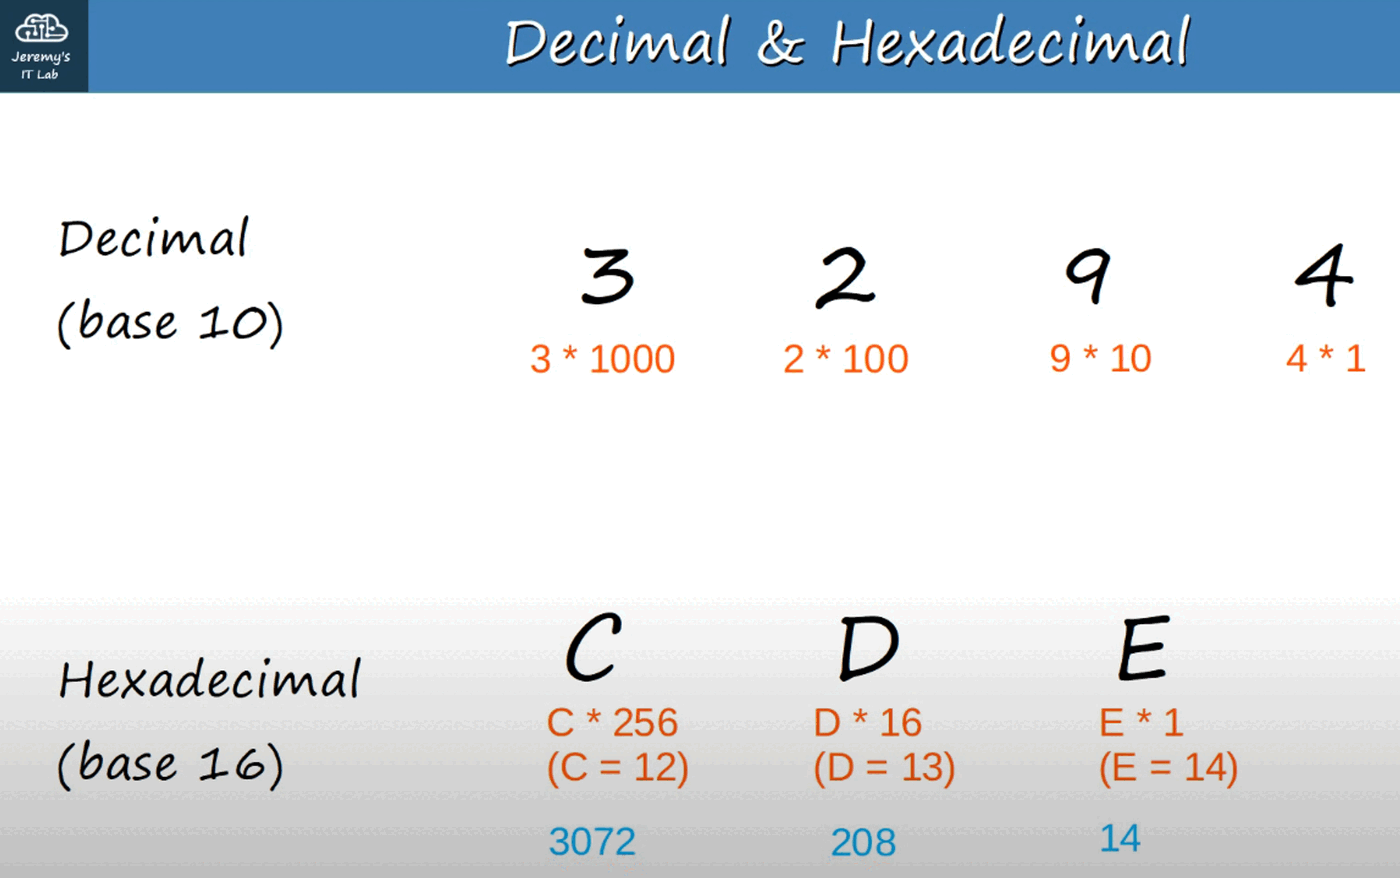
\includegraphics[keepaspectratio,alt={image}]{images/07-ipv4-addressing-part1/img-004.png}}
\end{figure}

Decimal (base 10)

Ex: 3294 = (3 * 1000) + (2 * 100) + (9 * 10) + (4 * 1)

Hexadecimal (base 16)

Ex: 3294, would be CDE

\begin{lstlisting}
C (C * 256 / 12 * 256 = 3072) // 256ths position
D (D * 16 / D=13 so 16*13 = 208) // 16ths position
E (E * 1 / E = 14)  // 1s position
\end{lstlisting}

Adding these up, we get 3294

So, how do we convert a BINARY NUMBER to a DECIMAL NUMBER? The same way
we convert to Hexadecimal.

10001111

So:

\begin{lstlisting}
1 * 128 = 128
1 * 8 = 8
1 * 4 = 4
1 * 2 = 2
1 * 1 = 1
\end{lstlisting}

Add them all up : 128 + 8 + 4 + 2 + 1 = 143

The answer is 143.

Another example:

01110110

\begin{lstlisting}
1 * 64 = 64
1 * 32 = 32
1 * 16 = 16
1 * 4 = 4
1 * 2 = 2
\end{lstlisting}

Add them all up: 64 + 32 + 16 + 4 + 2 = 118

The answer is 118.

Another example:

11101100

\begin{lstlisting}
1 * 128 = 128
1 * 64 = 64
1 * 32 = 32
1 * 8 = 8
1 * 4 = 4
\end{lstlisting}

Add them all up: 128 + 64 + 32 + 8 + 4 = 236

The answer is 236.

So, how do we convert a DECIMAL NUMBER to a BINARY NUMBER?

Take the number 221.

We can take that number and start subtracting it from LEFT to RIGHT of
our Binary slots.

221

\begin{lstlisting}
221 - 128 = 93 so we place a 1 in the "128" slot
\end{lstlisting}

10000000

\begin{lstlisting}
93 - 64 = 29 so we place another 1 in the "64" slot

29 - 32 isn't possible so we place a 0 in the "32" slot

29 - 16 = 13 so we place a 1 in the "16" slot

13 - 8 = 5 so we place a 1 in the "8" slot

5 - 4 = 1 so we place a 1 in the "4" slot

1 - 2 isn't possible so we put a 0 in the "2" slot

1 - 1 is possible so we put a 1 in the "1" slot
\end{lstlisting}

This, then, allows us to the write out the BINARY number for 221.

It is : 11011101

Another example: 127

\begin{lstlisting}
127 - 128 is not possible so 0 in "128"
127 - 64 is possible so 1 in "64"
63 - 32 is possible so 1 in "32"
31 - 16 is possible so 1 in "16"
15 - 8 is possible so 1 in "8"
7 - 4 is possible so 1 in "4"
3 - 2 is possible so 1 in "2"
1 is possible so 1 in "1"
\end{lstlisting}

So 127, in BINARY, is 0111 1111

Another example: 207

Alternatively, you can subtract the number from `255' (which is
1111111). The remainder, then, can be used to ``find'' where the 0's are
in the binary number.

255 - 207 = 48 so \ldots{}

1 1 0 0 1 1 1 1 (32 + 16 = 48)

11001111 is the correct answer.

IPv4 ADDRESSES

So we now know that IP Addresses are the Dotted Decimal conversion of a
series of BINARY NUMBERS (broken up into 4 OCTETS) like so:

192.168.1.254/24

But what does the /24 stand for?

\begin{figure}
\centering
\pandocbounded{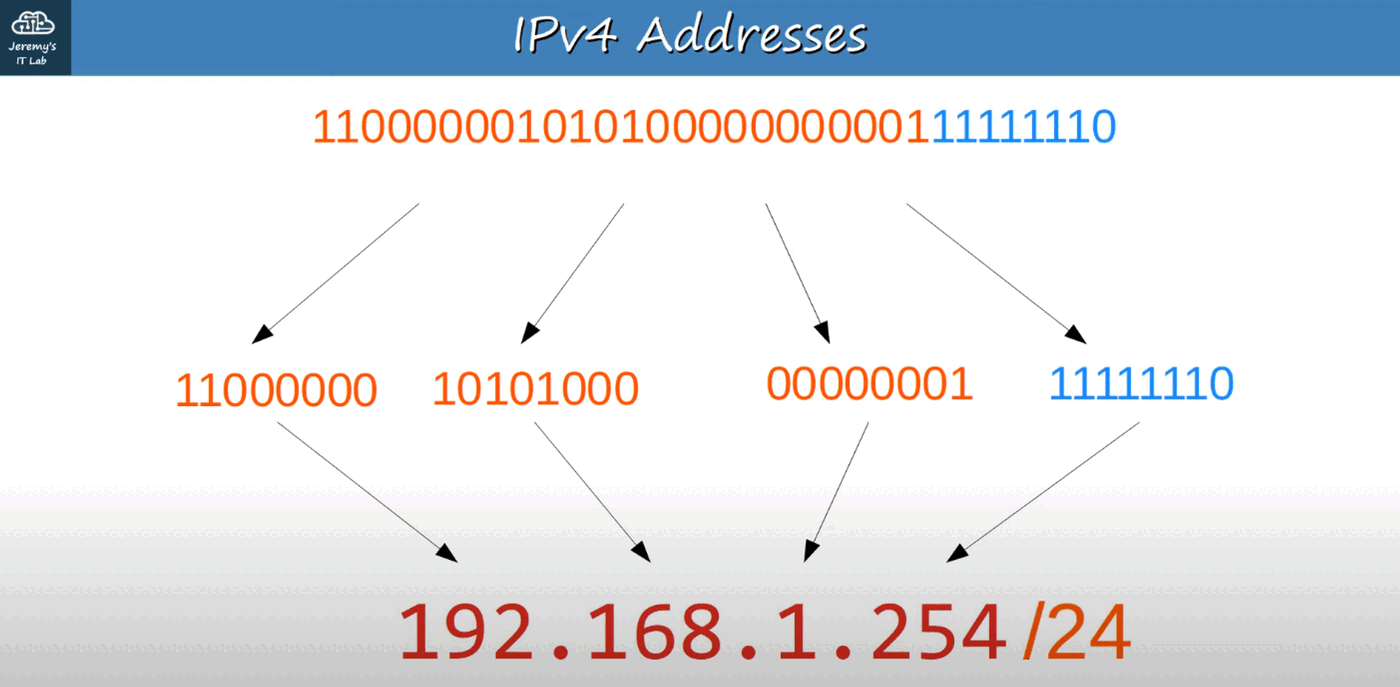
\includegraphics[keepaspectratio,alt={image}]{images/07-ipv4-addressing-part1/img-005.png}}
\end{figure}

It means the FIRST 24 BITS of this address represent the NETWORK portion
of the address.

192.168.1 is the NETWORK PORTION (the first 3 OCTETS)

.254 is the HOST PORTION (the last OCTET)

\begin{figure}
\centering
\pandocbounded{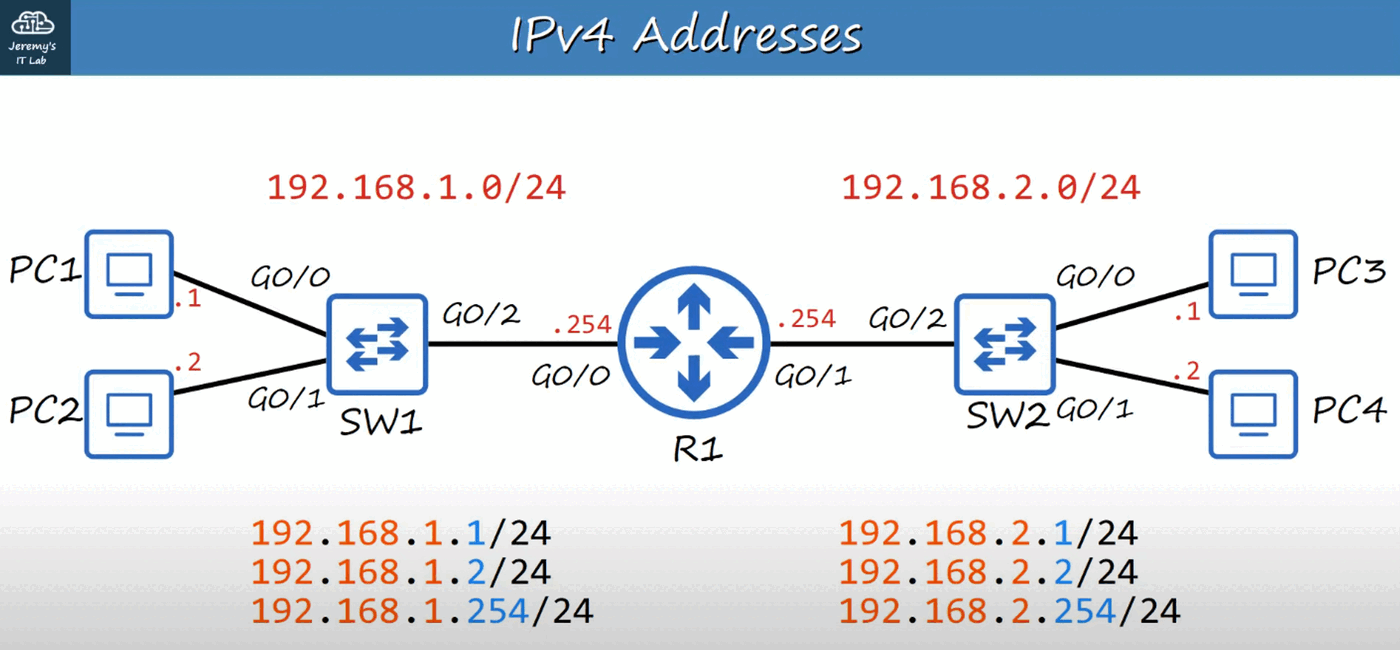
\includegraphics[keepaspectratio,alt={image}]{images/07-ipv4-addressing-part1/img-006.png}}
\end{figure}

CONVERT this BINARY number into an IPv4 Address:

10011010010011100110111100100000

10011010 . 01001110 . 01101111 . 00100000

Octets:

\begin{enumerate}
\def\labelenumi{\arabic{enumi}.}
\tightlist
\item
  128 + 16 + 8 + 2 = 154
\item
  64 + 8 + 4 + 2 = 78
\item
  64 + 32 + 8 + 4 + 2 + 1 = 111
\item
  32
\end{enumerate}

The IPv4 address is: 154.78.111.32/16

154.78 is the NETWORK PORTION 111.32 is the HOST PORTION

Another Example:

00001100100000001111101100010111

00001100 . 10000000 . 11111011 . 00010111

Octets:

\begin{enumerate}
\def\labelenumi{\arabic{enumi}.}
\tightlist
\item
  8 + 4 = 12
\item
  128
\item
  255 - 4 = 251
\item
  16 + 4 + 2 + 1 = 23
\end{enumerate}

The IPv4 address is: 12.128.251.23/8

12 is the NETWORK PORTION 128.251.23 is the HOST PORTION

IPv4 ADDRESS CLASSES

IPv4 ADDRESSES are split up into 5 different `classes'. The class of an
IPv4 is determined by the FIRST OCTET of the address.

\begin{lstlisting}
CLASS       FIRST OCTET         FIRST OCTET NUMBERIC RANGE

A            0xxxxxxx               0-126 + 127 'loopback'
B            10xxxxxx               128-191
C            110xxxxx               192-223
D            1110xxxx               224-239
E            1111xxxx               240-255
\end{lstlisting}

From the above chart, if the FIRST OCTECT STARTS with 0, the numeric
RANGE of possible first DOTTED DECIMAL is between 0-127.

The CLASSES we will be focusing on are CLASS A to CLASS C.

\begin{figure}
\centering
\pandocbounded{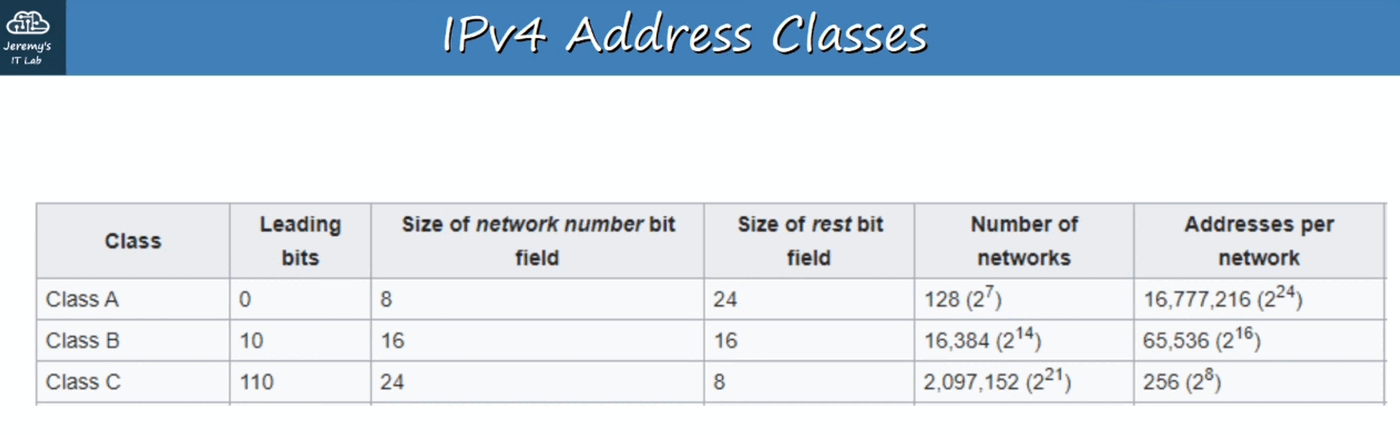
\includegraphics[keepaspectratio,alt={image}]{images/07-ipv4-addressing-part1/img-007.png}}
\end{figure}

D CLASS are reserved for `MULTICAST' ADDRESSES

E CLASS are reserved for `EXPERIMENTAL' ADDRESSES

A CLASS USUALLY have a range of 1-126? WHY?

Because 127 is usually reserved for `loopback addresses'

127.0.0.0 to 127.255.255.255 are used to test the network.

\begin{itemize}
\tightlist
\item
  Used to test the `Network stack' (OSI \& TCP/IP model) on the local
  device.
\end{itemize}

\begin{figure}
\centering
\pandocbounded{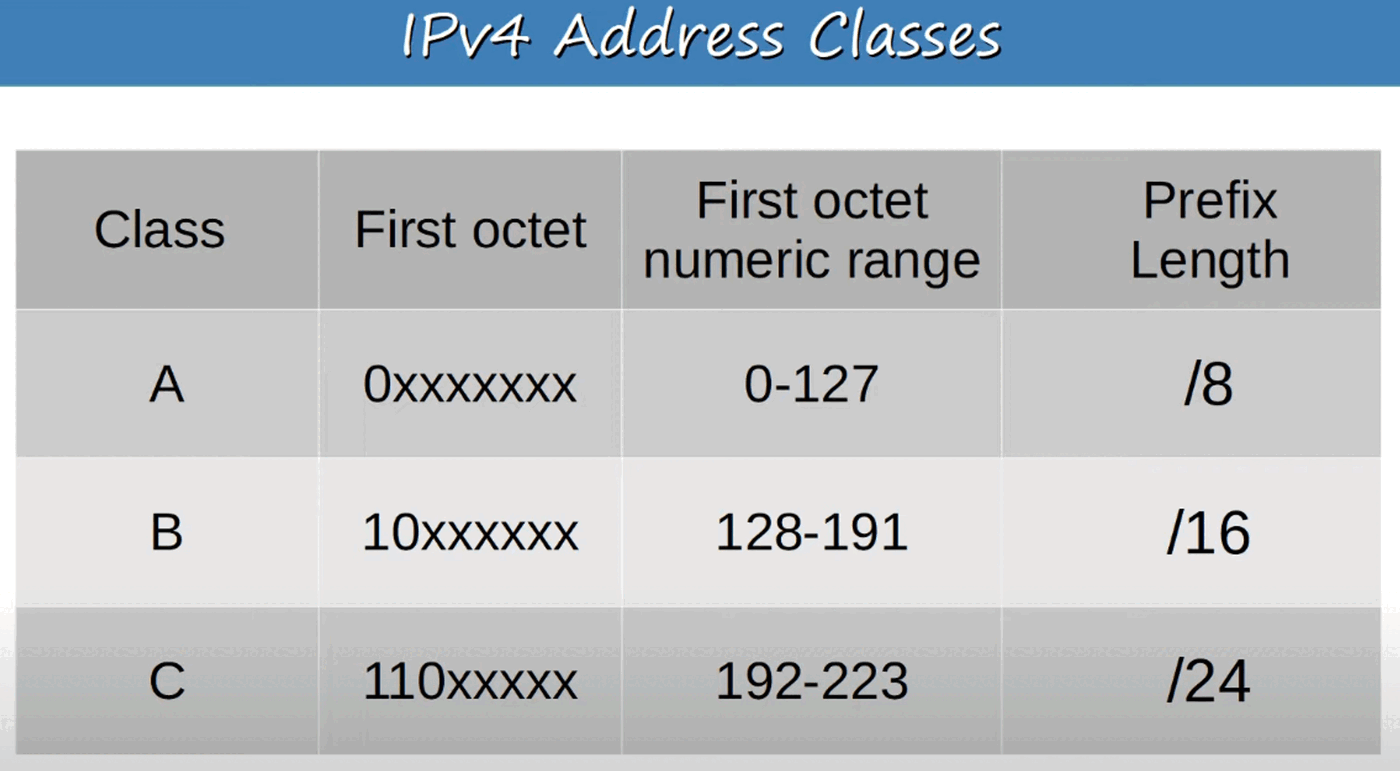
\includegraphics[keepaspectratio,alt={image}]{images/07-ipv4-addressing-part1/img-008.png}}
\end{figure}

The PREFIX LENGTH is the LENGTH of the NETWORK PORTION of the Address.

From the examples above:

12.128.251.23/8 is a CLASS A Address 154.78.111.32/16 is a CLASS B
Address 192.168.1.254/24 is a CLASS C Address

Because the NETWORK portion of CLASS A is so short, it means there are a
LOT more potential Hosts.

Because the NETWORK portion of CLASS C is so long, it means fewer
potential Hosts.

\section{Netmask}\label{netmask}

\begin{figure}
\centering
\pandocbounded{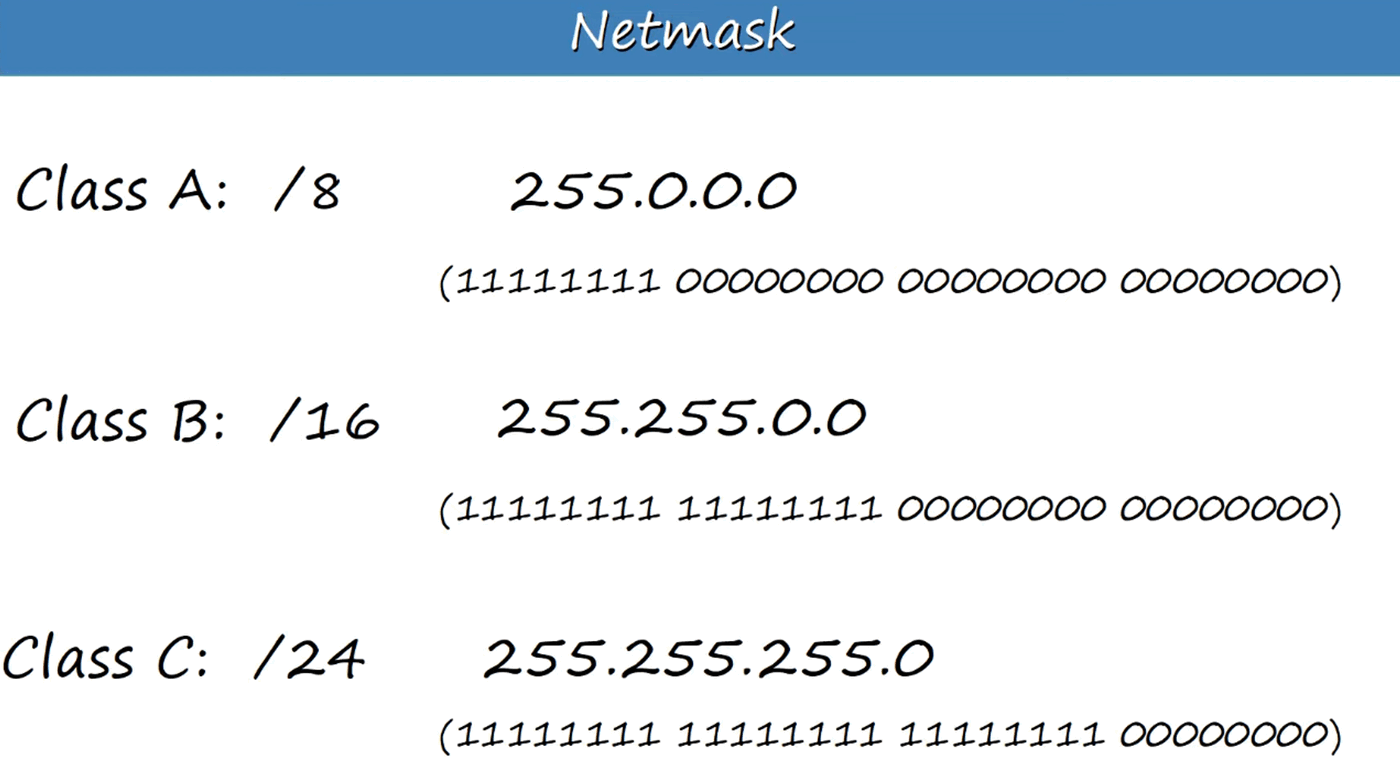
\includegraphics[keepaspectratio,alt={image}]{images/07-ipv4-addressing-part1/img-009.png}}
\end{figure}

A NETMASK is written like a Dotted Decimal IP Address

CLASS A: /8 = 255.0.0.0

CLASS B: / 16 = 255.255.0.0

CLASS C: /24 = 255.255.255.0

\section{Network Addresses}\label{network-addresses}

\begin{figure}
\centering
\pandocbounded{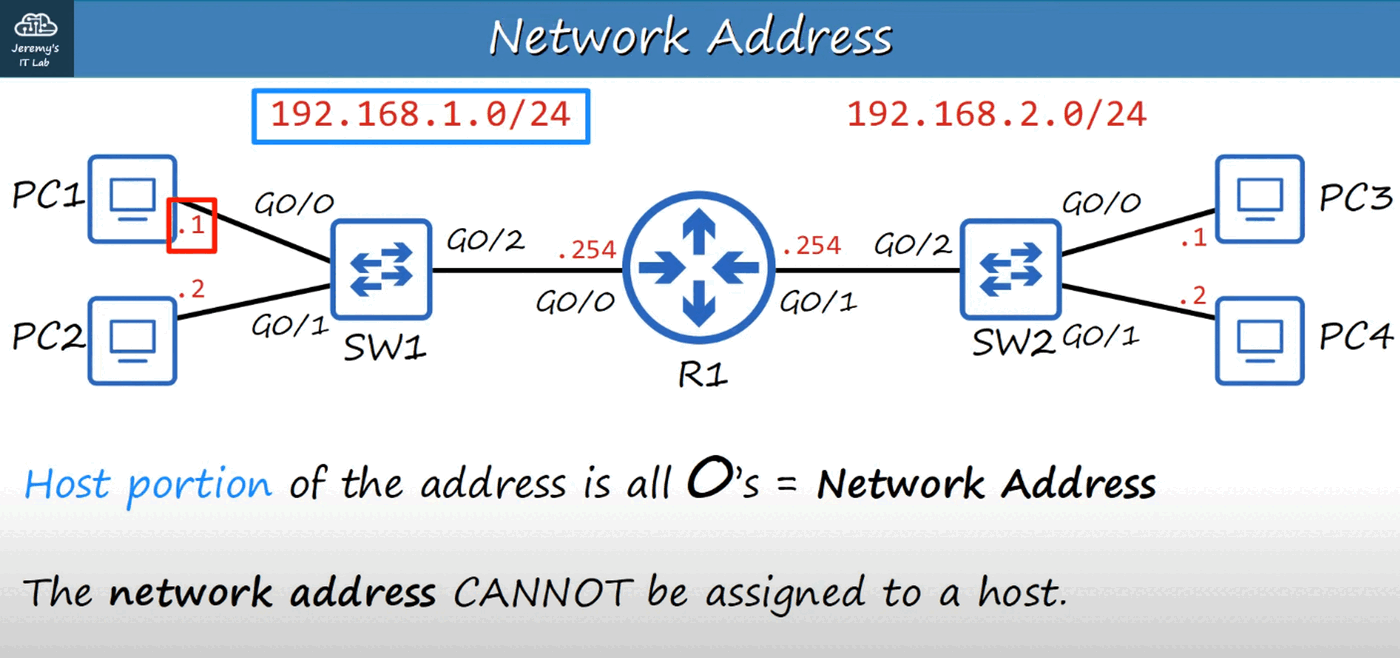
\includegraphics[keepaspectratio,alt={image}]{images/07-ipv4-addressing-part1/img-010.png}}
\end{figure}

If the HOST PORTION of an IP ADDRESS is ALL 0's, it means it is the
NETWORK ADDRESS = the identifier of the network itself.

Example: 192.168.1.0/24 = THIS is a NETWORK ADDRESS.

A NETWORK ADDRESS cannot be assigned to a HOST. A NETWORK ADDRESS is the
FIRST ADDRESS.

\begin{figure}
\centering
\pandocbounded{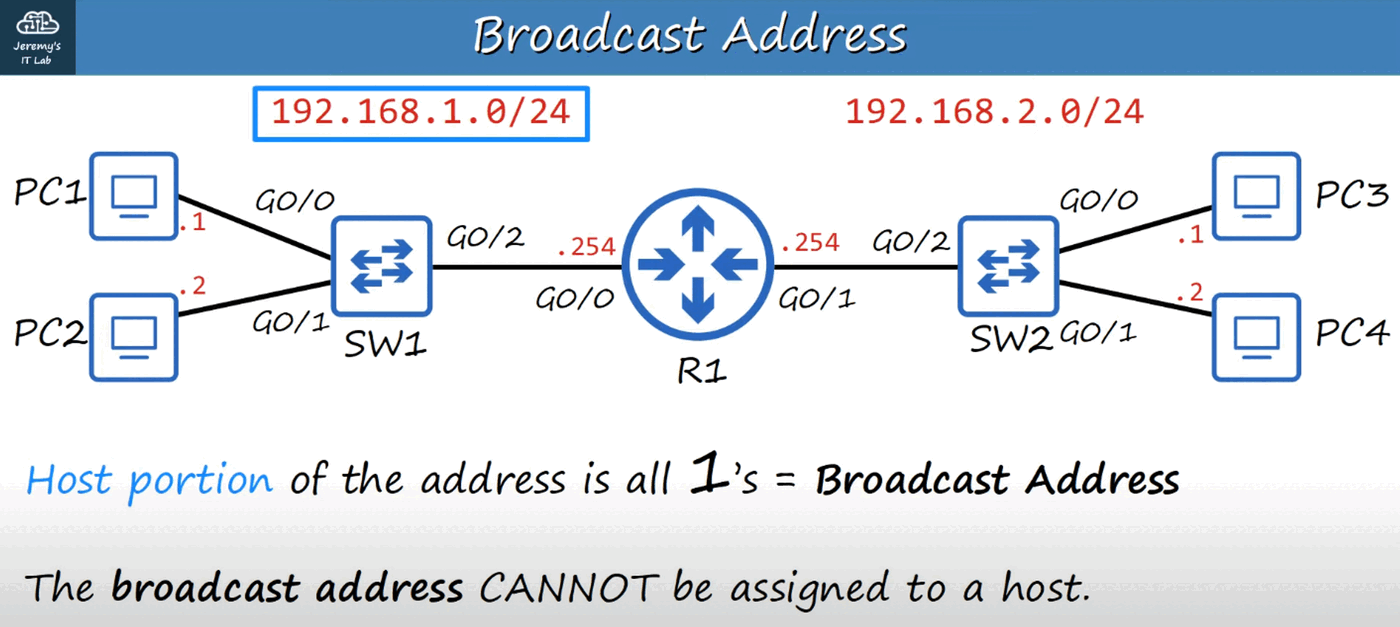
\includegraphics[keepaspectratio,alt={image}]{images/07-ipv4-addressing-part1/img-011.png}}
\end{figure}

If the HOST PORTION of an IP ADDRESS is ALL 1's, it means it is the
BROADCAST ADDRESS for the network.

A BROADCAST ADDRESS cannot be assigned to a HOST.

DESTINATION IP : 192.168.1.255 (Broadcast IP address) DESTINATION MAC :
FFFF.FFFF.FFFF (Broadcast MAC address)

Because of the two `reserved' addresses, the range of USABLE HOST
ADDRESSES is 1 to 254.
